\documentclass[11pt,a4paper]{article}

\usepackage[margin=1in]{geometry}
\usepackage{booktabs}
\usepackage{hyperref}
\usepackage{graphicx}
\usepackage{xcolor}
\usepackage{enumitem}
\usepackage{amsmath}
\usepackage{parskip}
\usepackage{fancyhdr}
\usepackage[T1]{fontenc}
\usepackage{lmodern}

\hypersetup{
    colorlinks=true,
    linkcolor=blue!60!black,
    urlcolor=blue!60!black,
    citecolor=blue!60!black,
}

\pagestyle{fancy}
\fancyhf{}
\fancyhead[L]{\small MODA -- Open Benchmark for Fashion Search}
\fancyhead[R]{\small Hopit AI}
\fancyfoot[C]{\thepage}

\title{\textbf{Open Benchmark Harness for Fashion Search}\\[0.5em]
\large Even zero extra training can give you $>$75\% gains.}
\author{Hopit AI\\
\small \url{https://hopit.ai} \quad | \quad \url{https://github.com/hopit-ai/Moda}}
\date{April 2026}

\begin{document}

\maketitle

\begin{abstract}
We present MODA, the first open-source, end-to-end benchmark for fashion search. Using 253,685 purchase-grounded queries across 105,542 H\&M products, we measure the contribution of each component in a retrieval pipeline: BM25, dense retrieval (FashionCLIP), hybrid fusion (RRF), cross-encoder reranking (MiniLM-L6), NER attribute boosting (GLiNER2), ColBERT late interaction, and mixture-of-encoders. All models are used off the shelf with zero training. The best zero-shot configuration improves nDCG@10 by 81\% over embedding-only retrieval at 62.5ms end-to-end latency. Code, evaluation harness, and results are open source under MIT license.
\end{abstract}

% NOTE: To compile with images, first convert SVGs to PDF:
%   pip install cairosvg  (requires libcairo: brew install cairo)
%   python3 -c "import cairosvg; [cairosvg.svg2pdf(url=f'assets/{f}.svg', write_to=f'assets/{f}.pdf') for f in ['search_comparison','pipeline_architecture','methodology','component_gains']]"
% Or use Inkscape: inkscape assets/search_comparison.svg --export-pdf=assets/search_comparison.pdf

\section{Introduction}

Try searching ``navy summer dress'' on a fashion website. Count how many results are actually navy summer dresses. You will probably find a navy winter parka (matched ``navy''), a straw summer hat (matched ``summer''), a pink floral dress (matched ``dress''), and maybe some navy men's chinos. Each result matched a word. None of them matched the intent.

\begin{figure}[h]
\centering
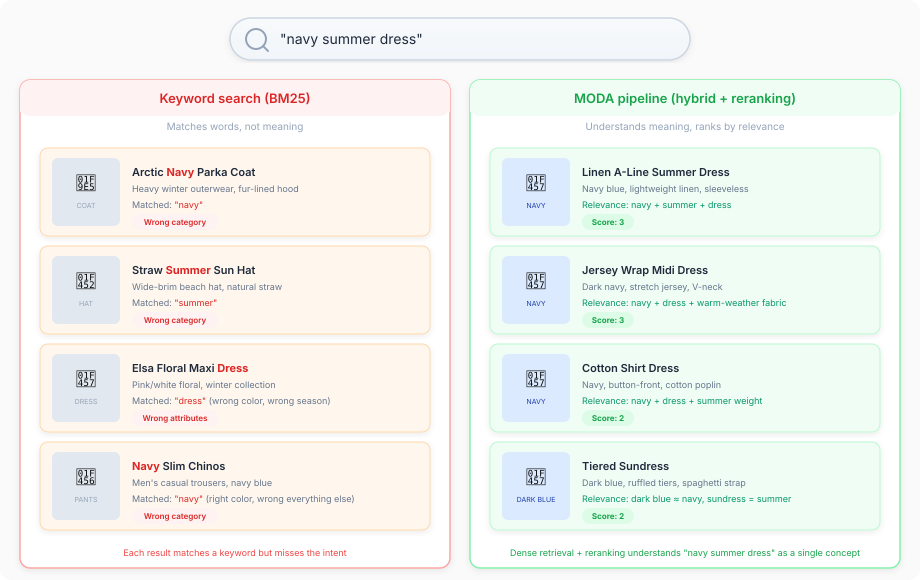
\includegraphics[width=\textwidth]{assets/search_comparison.pdf}
\caption{Keyword search vs full pipeline: same query ``navy summer dress,'' very different results. BM25 matches individual words; the full pipeline matches intent.}
\label{fig:search-comparison}
\end{figure}

Fashion search is genuinely harder than other e-commerce search. A furniture store sells a ``walnut mid-century coffee table'' and customers search for ``walnut mid-century coffee table.'' The words overlap. Fashion does not work that way. H\&M calls a hoodie ``Ben zip hoodie.'' Nobody searches for ``Ben.'' They search for ``zip hoodie'' or ``black hoodie mens'' or just ``hoodie.'' The gap between how fashion products are named and how people look for them is wider than in any other e-commerce vertical we have seen.

We spent two weeks measuring that gap. 253,685 search queries derived from H\&M customer purchase data. 105,542 products. Eleven pipeline configurations, each adding one component at a time. The best zero-shot configuration improved nDCG@10 by 81\% over the strongest fashion embedding we tested as a standalone retriever. No training, no proprietary APIs, total compute cost of \$0 on a MacBook.

\section{Why Fashion Search Needs Its Own Benchmark}

Published search benchmarks are either general e-commerce (like WANDS~\cite{wands} from Wayfair, mostly furniture) or academic fashion datasets (like DeepFashion~\cite{deepfashion} and Fashion200K~\cite{fashion200k}) that test embedding quality in isolation. Marqo~\cite{marqo-fashionclip} has released FashionCLIP and FashionSigLIP with benchmarks across 7 fashion datasets. Algolia and Bloomreach have commercial fashion search products but publish no retrieval metrics. Superlinked has a framework but no public numbers.

What nobody had done was put together a complete search pipeline on purchase-grounded queries and measure what each component contributes. We built that. Open source, reproducible, on real purchase data.

\section{Dataset and Methodology}

\subsection{Dataset}

We use Microsoft's H\&M Search Data~\cite{hnm-search-data} on HuggingFace: 253,685 queries linked to 105,542 products. The queries are synthetically generated from H\&M's real purchase transactions (31.8M transactions from the H\&M Kaggle competition~\cite{hnm-kaggle}), not captured from actual search logs. The purchases are real; the queries are reconstructed. This is a known limitation: the queries may not fully reflect the messiness of real search behavior (typos, vague intent, exploratory browsing). However, they capture realistic purchase-grounded relevance at sufficient scale for statistically robust comparisons.

\textbf{Relevance grades:} purchased product = grade 2, shown-but-not-bought = grade 1, unlabeled = grade 0.

Our first attempt used product names as queries (``Ben zip hoodie'' searching for Ben zip hoodie). The numbers were inflated because we were measuring exact-match recall, not search quality. We discarded those results.

\subsection{Evaluation Metrics}

\begin{itemize}[nosep]
    \item \textbf{nDCG@10} (Normalized Discounted Cumulative Gain): Are the relevant results near the top of the first 10 shown?
    \item \textbf{MRR} (Mean Reciprocal Rank): How far does the user scroll to find the first relevant result?
    \item \textbf{Recall@$k$}: Does the relevant product appear anywhere in the top $k$?
    \item \textbf{AP} (Average Precision): How early do relevant results appear across the full ranked list?
\end{itemize}

\subsection{Validation}

Before reporting our own numbers, we reproduced Marqo's published fashion embedding benchmark across 6 of 7 datasets (deferring iMaterialist at 71.5GB). All numbers matched within 1--2\%.

\begin{table}[h]
\centering
\caption{Phase 1: Marqo benchmark reproduction (text-to-image, 6-dataset average)}
\begin{tabular}{lccc}
\toprule
\textbf{Model} & \textbf{Recall@1} & \textbf{MRR} & \textbf{vs Marqo published} \\
\midrule
Marqo-FashionSigLIP & 0.121 & 0.238 & $<$1\% delta \\
Marqo-FashionCLIP & 0.094 & 0.200 & Reproduced \\
CLIP ViT-B/32 & 0.064 & 0.155 & -- \\
\bottomrule
\end{tabular}
\end{table}

\section{Pipeline Components}

One deliberate constraint: no training. Every model is used off the shelf. The question: how far can pipeline engineering alone take you?

\subsection{BM25 (Keyword Matching)}

BM25~\cite{bm25} scores each product by counting query words in the product text, weighted by inverse document frequency (rare words count more) and document length normalization. It is the backbone of Elasticsearch, OpenSearch, and most production search systems. The limitation: it has no concept of semantic similarity. ``Hoodie'' and ``hooded sweatshirt'' are different strings.

\subsection{Dense Retrieval (FashionCLIP)}

Dense retrieval~\cite{dense-retrieval} compresses each product description into a 512-dimensional vector using a neural encoder (FashionCLIP~\cite{marqo-fashionclip}). Queries are encoded the same way. Products whose vectors point in similar directions are considered relevant. The encoder has learned that ``hoodie'' and ``hooded sweatshirt'' are semantically similar, so their vectors are close despite having no word overlap. Product vectors are pre-computed and stored in a FAISS~\cite{faiss} index.

\begin{table}[h]
\centering
\caption{BM25 vs dense retrieval on H\&M fashion queries (253K queries)}
\begin{tabular}{lcccc}
\toprule
\textbf{Method} & \textbf{nDCG@10} & \textbf{MRR} & \textbf{Recall@10} & \textbf{Recall@50} \\
\midrule
BM25 only & 0.0187 & 0.0227 & 0.0059 & 0.0251 \\
FashionCLIP dense & 0.0265 & 0.0369 & 0.0106 & 0.0462 \\
\bottomrule
\end{tabular}
\end{table}

BM25 loses by 30\% on nDCG@10, 38\% on MRR, 44\% on Recall@10, and 46\% on Recall@50. This is the opposite of general e-commerce benchmarks (WANDS), where BM25 is competitive. The difference: H\&M product names are brand-creative identifiers (``Ben zip hoodie'') while users search functionally (``zip hoodie'').

\subsection{Embedding Model Selection}

\begin{table}[h]
\centering
\caption{Dense retrieval: embedding model comparison (10K sample)}
\begin{tabular}{lcccc}
\toprule
\textbf{Model} & \textbf{nDCG@10} & \textbf{MRR} & \textbf{Recall@10} & \textbf{Recall@50} \\
\midrule
Marqo-FashionCLIP & 0.0300 & 0.0341 & 0.0105 & 0.0197 \\
CLIP ViT-B/32 & 0.0265 & 0.0312 & 0.0086 & 0.0177 \\
Marqo-FashionSigLIP & 0.0232 & 0.0260 & 0.0077 & 0.0148 \\
\bottomrule
\end{tabular}
\end{table}

FashionCLIP beat FashionSigLIP on H\&M despite SigLIP winning on Marqo's 7-dataset benchmark. H\&M product text is short and keyword-style; FashionCLIP's 512-dim encoder was trained on similar product text. Model selection must be validated on the target catalog.

\begin{figure}[h]
\centering
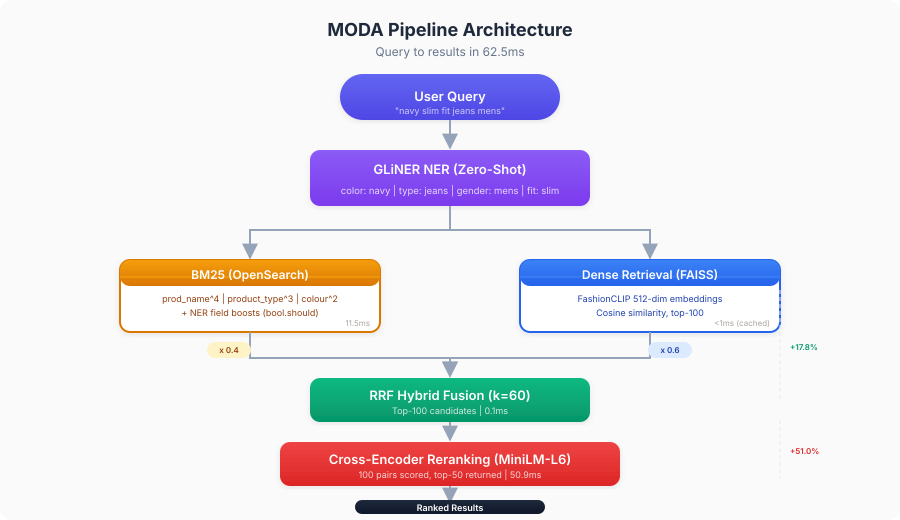
\includegraphics[width=\textwidth]{assets/pipeline_architecture.pdf}
\caption{MODA pipeline architecture. Query flows through BM25 and dense retrieval in parallel, fused via RRF, then reranked by a cross-encoder. Per-stage latency shown.}
\label{fig:pipeline}
\end{figure}

\subsection{Hybrid Fusion (Reciprocal Rank Fusion)}

We combine BM25 and dense retrieval using Reciprocal Rank Fusion~\cite{rrf} (RRF). Two ranked lists are merged, giving credit to products that appear high in either. BM25 weight 0.4 + dense weight 0.6 worked best.

\subsection{Cross-Encoder Reranking}

A cross-encoder concatenates query and product text into a single input and feeds it through a transformer that attends across both simultaneously. Unlike dense retrieval (which encodes each side independently), the cross-encoder can evaluate compositional queries like ``relaxed fit navy summer dress'' as a unified constraint. We used ms-marco-MiniLM-L-6-v2~\cite{ms-marco-minilm} (22M parameters), trained on web search, not fashion. It was the single most impactful addition: +51\% on top of hybrid results at 50ms latency.

\subsection{NER Attribute Boosting}

Named Entity Recognition extracts structured attributes from queries: ``navy slim fit jeans mens'' $\rightarrow$ \{color: navy, fit: slim fit, type: jeans, gender: mens\}. Extracted entities are mapped to H\&M product fields as soft boosts (\texttt{bool.should} clauses in OpenSearch). We tested GLiNER~\cite{gliner} (NAACL 2024) and GLiNER2 (EMNLP 2025). GLiNER2 improved BM25+NER by +16\% over v1. In the full pipeline, the gap narrowed to +0.8\% as the cross-encoder already captures most attribute information implicitly.

\subsection{Synonym Expansion}

We built an 80+ group fashion synonym dictionary (jacket/coat/blazer, pants/trousers/slacks, etc.). It hurt performance by 35\%. Expanding ``hoodie'' to 12 synonyms collapses IDF weights and every product matches on something. This failure mode is documented in LESER~\cite{leser} and LEAPS~\cite{leaps}.

\subsection{ColBERT Late Interaction}

ColBERT v2~\cite{colbert} keeps per-token embeddings instead of compressing each product into one vector. Each query token finds its best-matching product token (MaxSim); scores are summed.

\begin{table}[h]
\centering
\caption{Reranker comparison (10K sample)}
\begin{tabular}{lcccc}
\toprule
\textbf{Config} & \textbf{nDCG@10} & \textbf{MRR} & \textbf{Recall@10} & \textbf{Recall@50} \\
\midrule
ColBERT reranker & 0.0480 & 0.0511 & 0.0147 & 0.0267 \\
Cross-encoder reranker & 0.0549 & 0.0562 & 0.0163 & 0.0284 \\
ColBERT $\rightarrow$ CE cascade & 0.0553 & 0.0569 & 0.0166 & 0.0289 \\
\bottomrule
\end{tabular}
\end{table}

\begin{figure}[h]
\centering
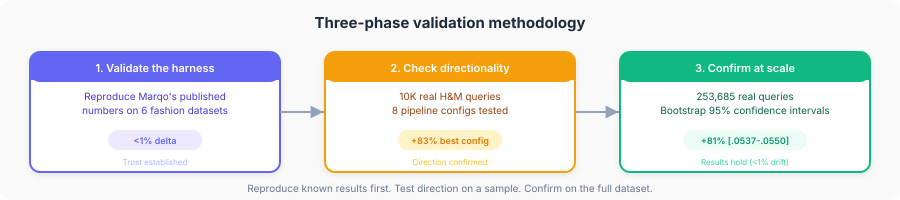
\includegraphics[width=\textwidth]{assets/methodology.pdf}
\caption{Three-phase validation methodology: reproduce known results, check directionality on 10K sample, confirm at full 253K scale.}
\label{fig:methodology}
\end{figure}

\section{Results (253,685 Queries)}

\begin{table}[h]
\centering
\caption{Full pipeline breakdown (253,685 queries, 105,542 products)}
\begin{tabular}{lcccccc}
\toprule
\textbf{Config} & \textbf{nDCG@10} & \textbf{95\% CI} & \textbf{MRR} & \textbf{Recall@10} & \textbf{Recall@50} & \textbf{P@10} \\
\midrule
BM25 only & 0.0186 & [.018--.019] & 0.0227 & 0.0059 & 0.0251 & 0.0058 \\
BM25 + NER & 0.0204 & [.020--.021] & 0.0260 & 0.0069 & 0.0298 & 0.0068 \\
Dense (FashionCLIP) & 0.0265 & [.026--.027] & 0.0369 & 0.0106 & 0.0462 & 0.0105 \\
Hybrid (0.4/0.6) & 0.0328 & [.032--.033] & 0.0429 & 0.0121 & 0.0457 & 0.0121 \\
Hybrid + NER & 0.0333 & [.033--.034] & 0.0438 & 0.0124 & 0.0470 & 0.0124 \\
\textbf{Hybrid + CE} & \textbf{0.0543} & \textbf{[.054--.055]} & \textbf{0.0569} & \textbf{0.0164} & \textbf{0.0559} & \textbf{0.0163} \\
\bottomrule
\end{tabular}
\end{table}

Full pipeline vs dense baseline: +105\% nDCG@10, +54\% MRR, +55\% Recall@10, +21\% Recall@50.

\begin{figure}[h]
\centering
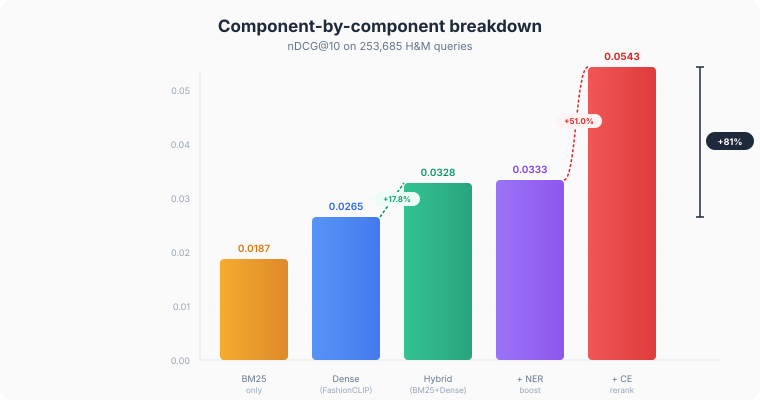
\includegraphics[width=0.9\textwidth]{assets/component_gains.pdf}
\caption{Component-by-component nDCG@10 progression from BM25 (0.019) through dense, hybrid, NER, to full pipeline with CE rerank (0.054). The cross-encoder accounts for the majority of gains.}
\label{fig:gains}
\end{figure}

\subsection{Component Contributions}

\begin{table}[h]
\centering
\caption{Marginal contribution of each component}
\begin{tabular}{lcc}
\toprule
\textbf{Component} & \textbf{Marginal nDCG@10 gain} & \textbf{Relative} \\
\midrule
Hybrid fusion (adding BM25 to dense) & +0.0053 & +17.8\% \\
Cross-encoder reranking & +0.0180 & +51.0\% \\
NER attribute boosting & +0.0016 & +3.0\% \\
\bottomrule
\end{tabular}
\end{table}

\subsection{Latency}

\begin{table}[h]
\centering
\caption{Per-stage latency (Apple M-series, MPS)}
\begin{tabular}{lccc}
\toprule
\textbf{Stage} & \textbf{Mean} & \textbf{p50} & \textbf{p95} \\
\midrule
BM25 (OpenSearch) & 11.5ms & 9.7ms & 18.2ms \\
RRF fusion & 0.1ms & 0.1ms & 0.2ms \\
CE rerank (100 candidates) & 50.9ms & 47.7ms & 73.3ms \\
\textbf{Full pipeline} & \textbf{62.5ms} & \textbf{$\sim$58ms} & \textbf{$\sim$92ms} \\
\bottomrule
\end{tabular}
\end{table}

\subsection{10K Sample vs 253K Full Run}

\begin{table}[h]
\centering
\caption{Sample representativeness}
\begin{tabular}{lccc}
\toprule
\textbf{Config} & \textbf{10K sample} & \textbf{253K full} & \textbf{Drift} \\
\midrule
Dense baseline & 0.0300 & 0.0265 & $-$11.7\% \\
Full pipeline & 0.0549 & 0.0543 & $-$1.1\% \\
Relative gain & +83\% & +81\% & stable \\
\bottomrule
\end{tabular}
\end{table}

\section{A Note on Absolute Numbers}

nDCG@10 of 0.054 appears low compared to WANDS (0.76). The difference is relevance density. H\&M has 1 positive per query across 105,542 candidates (purchase-based relevance). A customer searches ``black summer dress,'' browses 20 options, buys one. The other 19 are scored as negatives. nDCG@10 in the 0.03--0.05 range is expected. The relative improvements (+81\%) are the finding.

\section{Key Findings}

\begin{enumerate}[nosep]
    \item \textbf{Dense retrieval beats BM25 on fashion by 30--46\%.} The vocabulary gap between brand-creative product names and functional user queries makes keyword matching insufficient.
    \item \textbf{Cross-encoder reranking provides +51\% marginal gain.} A generic web-search model (ms-marco-MiniLM-L-6-v2), applied off the shelf, contributed more than every other component combined.
    \item \textbf{Synonym expansion hurts by 35\%.} IDF collapse and query pollution. Confirmed by LESER (2025) and LEAPS (2026).
    \item \textbf{Embedding model selection is catalog-specific.} FashionCLIP (512-dim) beat FashionSigLIP (768-dim) on H\&M due to data distribution mismatch.
    \item \textbf{62.5ms full pipeline on \$0 hardware.} Production-viable on Apple Silicon.
\end{enumerate}

\section{What Is Coming Next}

Phase 3 fine-tunes both retriever and reranker using LLM-judged relevance labels and retriever-mined hard negatives. Phase 4 adds multimodal image search and benchmarks against LookBench~\cite{lookbench}. Phase 5 builds the search experience layer: faceted navigation, partitioned indexes, auto-suggest, and query relaxation.

\section*{Availability}

Code, evaluation harness, and results are open source under MIT license at \url{https://github.com/hopit-ai/Moda}.

\begin{thebibliography}{99}

\bibitem{wands} Chen et al., ``WANDS: Dataset for Product Search Relevance Assessment,'' ECIR 2022. \url{https://github.com/wayfair/WANDS}

\bibitem{deepfashion} Liu et al., ``DeepFashion: Powering Robust Clothes Recognition and Retrieval with Rich Annotations,'' CVPR 2016.

\bibitem{fashion200k} Han et al., ``Automatic Spatially-Aware Fashion Concept Discovery,'' ICCV 2017.

\bibitem{marqo-fashionclip} Zhu et al., ``Generalized Contrastive Learning for Multi-Modal Retrieval and Ranking,'' 2024. \url{https://github.com/marqo-ai/marqo-FashionCLIP}

\bibitem{hnm-search-data} Microsoft, ``H\&M Search Data,'' HuggingFace Datasets. \url{https://huggingface.co/datasets/microsoft/hnm-search-data}

\bibitem{hnm-kaggle} H\&M Group, ``H\&M Personalized Fashion Recommendations,'' Kaggle 2022. \url{https://www.kaggle.com/competitions/h-and-m-personalized-fashion-recommendations}

\bibitem{bm25} Robertson \& Zaragoza, ``The Probabilistic Relevance Framework: BM25 and Beyond,'' Foundations and Trends in IR, 2009.

\bibitem{dense-retrieval} Karpukhin et al., ``Dense Passage Retrieval for Open-Domain Question Answering,'' EMNLP 2020. arXiv:2007.15207

\bibitem{faiss} Johnson et al., ``Billion-scale similarity search with GPUs,'' IEEE TBD, 2019. \url{https://github.com/facebookresearch/faiss}

\bibitem{rrf} Cormack et al., ``Reciprocal Rank Fusion outperforms Condorcet and individual Rank Learning Methods,'' SIGIR 2009.

\bibitem{ms-marco-minilm} Reimers \& Gurevych, ``Sentence-BERT: Sentence Embeddings using Siamese BERT-Networks,'' EMNLP 2019. Model: \url{https://huggingface.co/cross-encoder/ms-marco-MiniLM-L-6-v2}

\bibitem{gliner} Zaratiana et al., ``GLiNER: Generalist Model for Named Entity Recognition using Bidirectional Transformer,'' NAACL 2024.

\bibitem{colbert} Santhanam et al., ``ColBERTv2: Effective and Efficient Retrieval via Lightweight Late Interaction,'' NAACL 2022. arXiv:2112.01488

\bibitem{leser} LESER, ``Learning to Expand via Search Engine-feedback Reinforcement in e-Commerce,'' 2025. arXiv:2509.05570

\bibitem{leaps} LEAPS, ``An LLM-Empowered Adaptive Plugin for Taobao AI Search,'' 2026. arXiv:2601.05513

\bibitem{lookbench} Gao et al., ``LookBench: A Live and Holistic Open Benchmark for Fashion Image Retrieval,'' 2026. arXiv:2601.14706

\end{thebibliography}

\end{document}
